\documentclass[conference]{IEEEtran}
\IEEEoverridecommandlockouts
% The preceding line is only needed to identify funding in the first footnote. If that is unneeded, please comment it out.
\usepackage{cite}
\usepackage{amsmath,amssymb,amsfonts}
\usepackage{algorithmic}
\usepackage{graphicx}
\usepackage{textcomp}
\usepackage{xcolor}

\ifCLASSOPTIONcompsoc
    \usepackage[caption=false, font=normalsize, labelfont=sf, textfont=sf]{subfig}
\else
\usepackage[caption=false, font=footnotesize]{subfig}
\fi

\usepackage{siunitx}


% begin DWei added #1
\usepackage{fancyhdr}
\fancyhf{} % comment this to show page number on center footer
\pagestyle{fancy}
\rfoot{\parbox{3.5in}{\raggedleft\fontsize{8pt}{10pt} \selectfont \textcolor{gray}{The 9th Asia-Pacific International Symposium on Advanced Reliability and Maintenance Modeling  (APARM 2020 -- Vancouver)}}}
% end DWei added #1

\def\BibTeX{{\rm B\kern-.05em{\sc i\kern-.025em b}\kern-.08em
    T\kern-.1667em\lower.7ex\hbox{E}\kern-.125emX}}
\begin{document}

\title{A PdM Framework Through the Event-based Genomics of Machine Breakdown*\\
\thanks{This project has received funding from the European Union's Horizon 2020 research and innovation program under grant agreement Nos 768869 (Z-BRE4K) and 723906 (Z-FACT0R).}
}

\author{\IEEEauthorblockN{Morad Danishvar}
\IEEEauthorblockA{\textit{College of Engineering, Design and} \\ \textit{Physical Sciences} \\
\textit{Brunel University}\\
London, UK \\
Morad.Danishvar@brunel.ac.uk}\\
\and
\IEEEauthorblockN{Veerendra C. Angadi}
\IEEEauthorblockA{\textit{College of Engineering, Design and} \\ \textit{Physical Sciences} \\
\textit{Brunel University}\\
London, UK \\
Veer.Angadi@brunel.ac.uk}\\
\and
\IEEEauthorblockN{Alireza Mousavi}
\IEEEauthorblockA{\textit{College of Engineering, Design and} \\ \textit{Physical Sciences} \\
\textit{Brunel University}\\
London, UK \\
Alireza.Mousavi@brunel.ac.uk}\\
}

\maketitle
% begin DWei added #2
\thispagestyle{fancy}
% begin DWei added #2

\begin{abstract}
A novel event-based predictive maintenance framework based on sensor signal measurements and regressive predictions to minimise machine breakdown and component failure is proposed. Such capabilities will be complemented by Event-Clustering technique to cluster and remove less impact sensor signals and also build breakdown genomics from the root of a failure in order to predict the upcoming machine breakdowns and components failures.  The creation of machine breakdown genomics requires the knowledge of systems state observed as well as the state change at specified time intervals (discretization). The proposed framework is applied to a real application case study. An industrial case study of a continuous compression moulding machine that manufactures the plastic bottle closure (caps) in the beverage industry has been considered as an experiment. The machine breakdown genomics theory is tested in this case to build the sequence of events or the genomics of breakdown, where sequences of contiguous events lead to failure or healthy machine status. This is complemented by the Regression Event-Tracker method to estimates the condition monitoring of the components and provide components real-time remaining useful life estimation. The Weibull failure-rate analysis is carried out on the remaining useful life estimates for each element to understand and estimate the mean time to failure for the manufacturing machine.

\end{abstract}

\begin{IEEEkeywords}
Real-time Event Sequencing, Genomics of Machine Breakdown, Predictive Maintenance, Regressive Event Tracker, RUL, Machine Learning, Compression Moulding Machine
\end{IEEEkeywords}


\section{Introduction}
\label{sec:Introduction}
Over the last decades, there have been considerable advances in integrated sensors, instrumentation, signal processing algorithms, and internet technology infrastructure that lead the concept of smart factories under the concept of “Industry 4.0”. It has been estimated that already, \numrange{26}{50} billion ``things" are connected to the Internet, and this means the creation of a huge online amount of data \cite{Kumar2019}. This concept instigates today's increasing large-scale developments in machinery health monitoring.  Machinery health monitoring includes three stages of fault detection, fault diagnosis, and remaining useful life (RUL) prediction which the latter is an essential requisite for proactive maintenance and prognostic health management (PHM) \cite{Jin2019}. RUL prediction is a process using predictive methods to forecast the upcoming performance of machinery and obtain the time left before the machine loses its capabilities in operation \cite{Zhao2015}. Predictive Maintenance (PdM) is one of the most critical components of smart manufacturing and Industry 4.0 \cite{Calabrese2019}.  The benefits of PdM include improved efficiency, quality and safety, better compliance and mainly costs reduction due to prevention of machines and equipment damages. PdM strategy for industrial equipment can accurately perceive performance degradation since it was designed to achieve near-zero breakdowns throughout the entire manufacturing process \cite{Zhang2019}. Therefore, the Industrial Internet of Things (IIoT) revolution combination with today's advanced data analytical methods, enable industries to implement new and more effective maintenance strategies to progress the PdM. This instigates the authors to present a novel approach for sequential learning of breakdown’s events in industry domain. The named Genomic of machine breakdown (GMB) terminology borrows some of the classical term and descriptors of DNA sequencing from biology science to prognosis the upcoming breakdowns or components failure. Furthermore, a regression-based event-tracker is introduced to the estimate of the RUL and Mean time to failure (MTTF) of the machine in real-time by exploiting the event-clustering and genomics of the failure. In the following sections, a review of the most relevant PdM methods available in the literature is presented, followed by a detailed description of the proposed GMB and Regressive Event-Tracker methods and their applications in an industrial case study.

\section{Related Works}
\label{sec:Related_works}
In the recent years, extensive research works have been conducted in the subject of PdM and PHM (including fault and breakdown prognosis and RUL) in manufacturing industry domain. For example, reference \cite{Xia2018} addresses recent research works in PHM for advanced manufacturing paradigms to forecast health trends, avoid production breakdowns, reduce maintenance cost and achieve rapid decision making. Availability of large dataset of machines status and process parameters, as well as advancements in signal processing techniques, are the main reason for these extensive research works \cite{Susto2015}. PdM methods in the literature are mainly classified into four categories of model-based, knowledge-based, data-driven and hybrid prognosis \cite{Liao2014}. However, between these methods, data-driven PdM extensively applied to industrial manufacturing using methods such as time series \cite{Lin2019}, principle component analysis (PCA) \cite{You2015}, the hidden Markov model (HMM) \cite{Vrignat2015}, neural network \cite{Malhi2011}, machine learning (ML) \cite{Jiang2018,Carvalho2019} and deep learning (DL) algorithms \cite{Namuduri2020,Li2019a}. The ML-based PdM is divided into the two main classes of supervised, where the failures' information is known (e.g. regression method in \cite{Kumar2019} and classification method in \cite{Canizo2017}) and unsupervised, where only process information is available. But, maintenance data are not available \cite{Jiang2018}. The solutions provided by supervised learning are accurate, but the availability of maintenance information is strictly related to the adopted maintenance management policy. The authors of reference \cite{Lei2018} have conducted a comprehensive review on data-driven approaches applied in recent years in PdM domain. Another recent comprehensive review has been conducted in \cite{Zhang2019} on PdM applications from the aspects of ML and DL. This research also compared and ranked the methods based on their accuracy. Reference \cite{Werner2020,Aivaliotis2019} presents a methodology to calculate the RUL of machinery equipment by utilizing physics-based simulation models and digital twin concept to enable PdM for manufacturing resources using PHM techniques. The PHM aims to predict the RUL of the machine from the historical and ongoing degradation trends obtained from condition monitoring information. In the past years, a large number of research works have been conducted specifically on RUL prediction approaches which been divided into four groups according to their techniques and methodologies: physics model-based, statistical-based, hybrid and ML-based methods \cite{Jiang2018,Aivaliotis2019,Li2020}. Physical model and statistical-based methods use empirical physical and mathematical models of failure mechanisms to interpret machine breakdown and degradation trends \cite{Cai2020,Zhang2020,Ahmad2019}. A disadvantage of conventional statistical modelling approaches is that they rely on expert prior knowledge, heuristic decision and several assumptions. Other examples of research delivered in RUL estimation domain are recurrent neural network (RNN) in \cite{Guo2017}, Wiener-process-based methods in \cite{Zhang2018} and HMM in \cite{Chen2019}. Another method in RUL prediction is an ensemble learning based prognostic method \cite{Li2019b}. This research work combines multiple deep learning algorithms to predict more accurately. However, deep learning drawback is it’s highly reliance on the availability of large training dataset, while in real-world applications, despite the availability of large dataset of a normal operational dataset, it is often impossible to obtain a significant number of failure or breakdown dataset sample. Therefore, these deep neural network methods are not able to cover the major challenge in data-driven prognostics: Prediction of rare failures and breakdowns in PdM and RUL estimation. With reference to the constituent nodes of the Markovian processes chain which form a series of sequences akin to genes terminology in the DNA which are repeatable and predictable, an online temporal sequence learning algorithm named GMB technique is introduced in the next section. The proposed technique learns the event of complex sequencing in real-time while existing types of learning (such as statistical and ML) methods are not well suited to solve such real and practical need and desire from industrial applications.

\section{Sequential Breakdown Prediction the Theory of Event-Base GMB}
\label{sec:GMB}
The intention here is to develop an accurate and applicable machine breakdown predictive framework that be able to predict upcoming anomaly machine breakdown and estimate the components useful life. So that during the process, the online likelihood of breakdowns is identified, the system is alerted, and subsequently, prognostic maintenance is taken, these leads to zero-break manufacturing. As reviewed in the previous section, all learning-based methods require training and large sets of data that rarely exists about the state of the machine and the type of breakdown. Furthermore, no formal and verifiable data/knowledge exists of the correlations between systems parameters that relate to machine breakdown. The challenge was to build a real-time machine breakdown framework that is able to interlink the causal relationship between machine parameters/state and its maintenance schedule and remaining life-time. This prediction and appropriate taking action mean savings of machine life and improvement in the machine performance and quality of the products. The proposed method introduces a general framework for using Event-Clustering technique \cite{Danishvar2018} and event sequence prediction (ESP) in forming a GMB terminology. The ESP consists of predicting the occurrence of the next elements of a sequence based on the sequential nature of events and previously observed elements. Event sequencing is, registering as an observed event at specified time intervals. If such occurrence has not been observed previously, then a new event is registered. We have named the proposed method as a theory of event-based genealogy of breakdown since this prediction method borrows its terminology from genetics science. Similar to the chains in a DNA, the sequences of events are representing machines parameters and states causal relationships. The strings in the DNA of a machine breakdown can be presented the linear sequence of events where a specific constellation can be interpreted as the building blocks of the breakdown. For example, the chain of events that forms the DNA of a healthy machine that successfully produces a ``non-defective product" or otherwise. Some constellations of machine's genes (DNA) will lead to ``non-defective" products and some lead to defects. Eventually, recognising and identifying and labelling the machine defect genes will lead to prognosis the cause and life-time of the machine breakdown. Moreover, identifying the machine breakdowns' genes will help to take maintenance actions. In this paper, an example of manufacturing where the GMB type 1 is presented as a sequence and chain of events (genes labelled alphabetically) that prognosis state of the machine breakdown one is discussed. For instance, the first breakdown can be labelled as a combination of repeatable events labelled A, B, C, D, and this breakdown would happen if a sequence of A$\to$B$\to$C$\to$D occurs. A, B, C, D are representative of distinguished machine states which will be explained in detail in the next sections.

\subsection{GMB Algorithm}
\label{subsec:GMB_Algorithm}
The proposed GMB methods begin with dimensionality reduction through Rank Order Clustering (ROC) technique to ranks and groups the relationship between machine input and output parameters \cite{Danishvar2018}. The array of inputs and their weight vis-à-vis system outputs are used in building the event sequences genomes blocks and their likelihood of occurrence. The following step is the definition of a safety threshold (ST). This threshold is defined by the manufacturer for the operational reasons or as a limit of operations. As the sensor values cross the ST a breakdown may not occur; however, the machine is not operating in the optimum performance level.
\begin{figure}[t]
\centerline{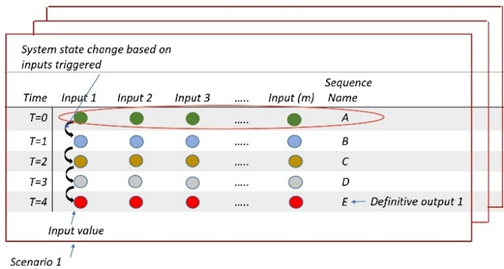
\includegraphics[width=0.7\linewidth]{Genome_Labelling.png}}
\caption{Genome labelling and sequential differentiation example.}
\label{fig:Genome_labelling}
\end{figure}
Genomes labelling and sequential event differentiation is the next step in GMB training algorithm. In this step, detection of the state of the machine is conducted at every collected sample, and then each detected state is labelled as illustrated in Fig.~\ref{fig:Genome_labelling} to generate the sequence of breakdown. Here, in this example, the breakdown threshold is at $T = 4$. Then the value of relevant sequences will be read and labelled in the following time sequences of $t0$, $t1$, $t2$, $t3$, $t4$. To generate the sequence of ABCDE to prognosis the machine breakdown. In this example, the genome length is five elements. The first element in the sequence is registered at $t0$ and labelled as `A', then according to the clustering output which ranks the inputs importance weight on the outputs, the second sequence labelled could be a new state differentiable to the prior state, only if the system state's difference passes the trigger threshold (see \cite{Tavakoli2013} to trigger threshold definition) then a new label is assigned to the new state as `B' this is continued until the moment of state `E' which is occurrence at breakdown threshold. Subsequently the formation of events from $t0$ to $t4$, five consecutive events form the genome strand `ABCDE'.
At the end of the training, all trained genomes will be stored in the sequence database as a lookup table to predict different machine breakdown scenarios. In the above example, if during prediction, state `A' is detected, the likelihood of the breakdown is $20\%$ (one out of five possible events). Consequently, if `A'$\to$`B'$\to$`C'$\to$`D' occurred in the real-time prediction, more likely the next sequence is `E' unless it occurred otherwise.
A case study is presented in the following section to explain further the implementation of the GMB in a real industrial case. Here every step of the machine breakdown is registered in the form of a chain of events coded in the form of a sequence of genomes representing the DNA of machine that lead to ``healthy" or ``breakdown" outcome.

\section{The DNA of continuous compression machine}
\label{sec:DNA_CCM}
A use case of a continuous compression moulding machine is considered which manufactures the plastic bottle closure (caps) that caters for the beverage industry. The process uses a compression moulding technique rather than the more traditional approach of injection moulding machine \cite{Liu2020}. The compression moulding \cite{Peltonen1992} machine produces bottle caps at a faster rate with the process of compressing and cooling happening at the same stage. The crucial process in the manufacturing of the caps is the coolant which is cooling the moulded plastic. This module is called the thermal regulator. The thermal regulator maintains the temperature of the coolant through the process by a series of a control system, as shown in Fig.~\ref{fig:TH_schematic}.
\begin{figure}[b]
\centerline{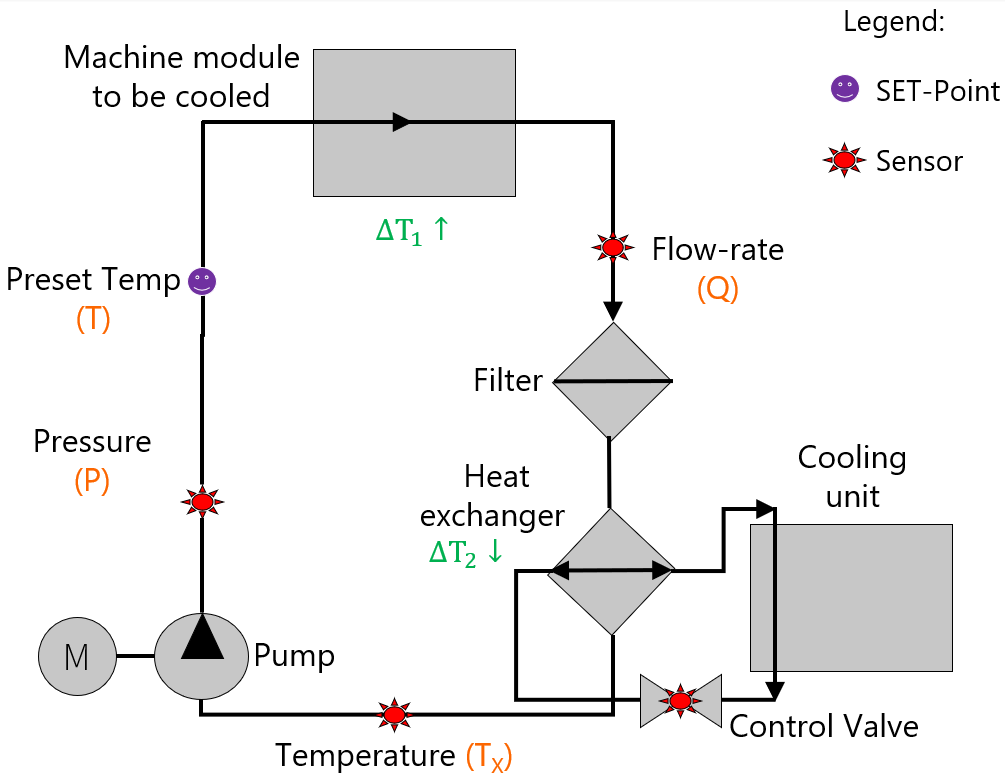
\includegraphics[width=0.5\linewidth]{TH_schematic.png}}
\caption{The flow diagram of the coolant in the thermal regulator.}
\label{fig:TH_schematic}
\end{figure}
The coolant temperature is set by the operator, which is customised and the recipe of the desired caps manufacturer. The set values of temperature ($T$) are maintained by the combinations of pumps and heat exchanger. The coolant passes through the module which has the molten plastic, which is to be cooled. The temperature of the coolant gains the temperature of $\Delta T_1$ after passing through the heat source. The coolant then passes through the filter so that the particulates (if any) are filtered and then to a heat exchanger. The heat exchanger reduces (by $\Delta T_2$) the coolant temperature back to the set temperature ($T$). The values of $\Delta T_1$ and $\Delta T_2$ are maintained equally to retain $T$ value.
The health of thermal regulator is monitored by the four sensors, i.e. Temperature ($T_x$), pressure ($P$), coolant flow-rate ($Q$) \& valve control. The proprietary sampling rate of the sensor acquisition is every cycle of the manufacturing of caps. The temperature ($T_x$) is used in the feedback mechanism for the heat exchanger to maintain the constant coolant temperature at $T$. The control values are used to chill more of the coolant if the $T_x>T$. The presence of the filter decreases the flow-rate of the coolant in the circuit. This is an indicator of the degradation of the filter. The failure mode evaluation and critical analysis (FMECA) reports reveal that the filter clog is the main failure mode involving a repeated change of the filters over time due to the clogs. The clogs in the filter are due to the suspended particulates in the coolant, which decreases the flow-rate. This decrease in flow-rate causes motor to pump more coolant into the circuit, causing an increase in pressure ($P$). The dynamics of the flow-rate ($Q$) and pressure ($P$) are shown in Fig.~\ref{fig:QP_relation}. The coolant flow-rates values are the direct impact of the continuous filter clogging over time. Fig.~\ref{fig:Sensor_values} indicates that the machine has been stopped and preventive maintenance has been carried to clear the filter.
%\begin{figure}[htbp]
%\centerline{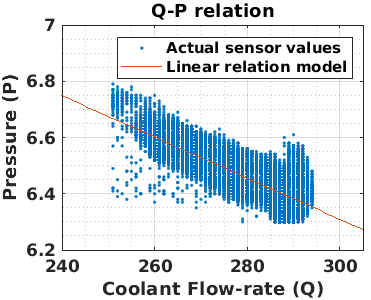
\includegraphics[width=0.7\linewidth]{QP_relation.png}}
%\caption{The control system feedback relation between coolant flow-rate ($Q$) and the %pressure ($P$).}
%\label{fig:QP_relation}
%\end{figure}
%\begin{figure}[htbp]
%\centerline{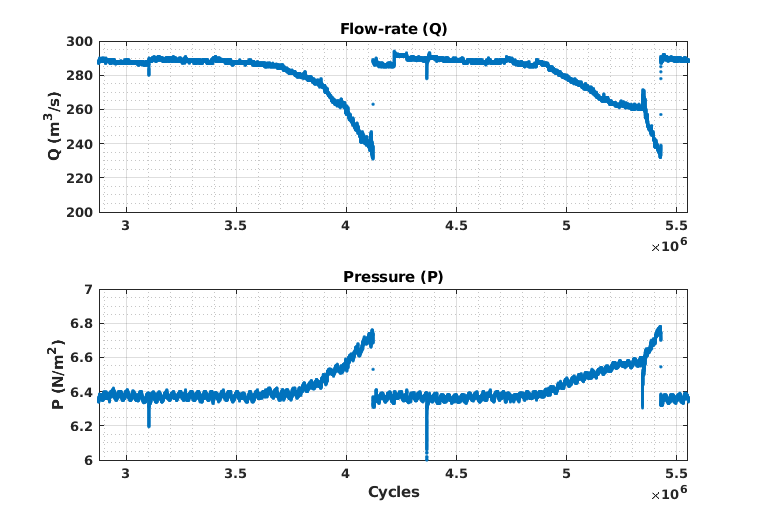
\includegraphics[width=0.7\linewidth]{Sensor_values.png}}
%\caption{The coolant flow-rate and pressure sensor values after performing preventive %maintenance by clearing the clogs in the filter.}
%\label{fig:Sensor_values}
%\end{figure}
\begin{figure}[t]
    \centering
    \subfloat[\label{fig:QP_relation}]{%
       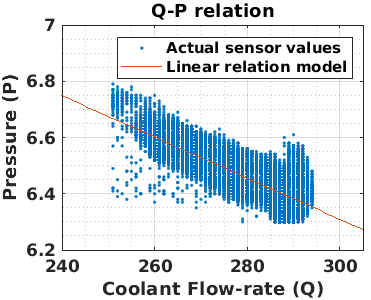
\includegraphics[width=0.5\linewidth]{QP_relation.png}}
    \hfill
  \subfloat[\label{fig:Sensor_values}]{%
        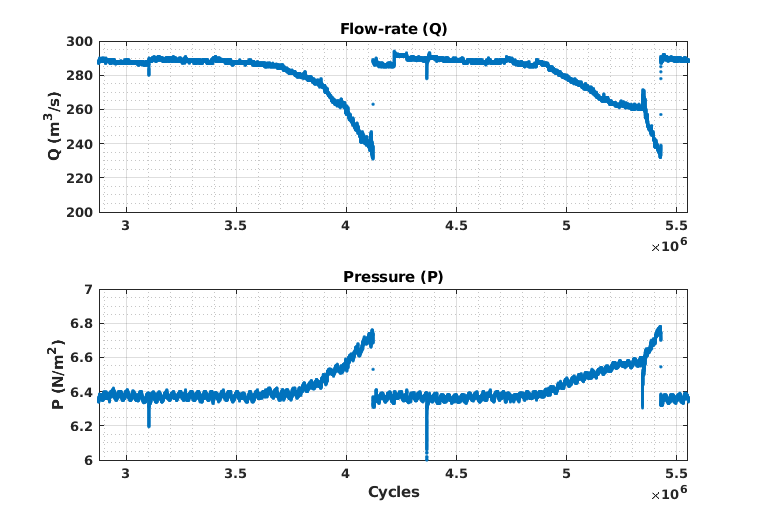
\includegraphics[width=0.5\linewidth]{Sensor_values.png}}
    \caption{(a) The control system feedback relation between coolant flow-rate ($Q$) and the pressure ($P$). (b) The coolant flow-rate and pressure sensor values after performing preventive maintenance by clearing the clogs in the filter.}
\end{figure}
The step-by-step implementation of the proposed ESP is as follows:

\subsection{Event-Clustering sensitivity analysis algorithm}
\label{subsec:event_clustering}
As explained above, GMB algorithm begins with dimensionality reduction through Event clustering technique. This helps to find the correlation between inputs and output signal parameters, reveals the sensitivity of the filter clogging (output) against the machine state parameters (system input signals i.e. coolant flow-rate, pressure, control valve and temperature). The interpretation of the data series is based on triggers and events. Only those changes in the data series that are interpreted as triggers represent state change, and the trigger threshold was set at $2\%$ (chosen by conducting a false negative test and system expert \cite{Tavakoli2013}). It means that any alteration in input sensors (machine data) and filter clogging, more than $2\%$ has been considered as a new event. The Event-Cluster outputs are shown in Table~\ref{tab:I}.
\begin{table}[b]
    \caption{Event Clustering output between the machine sensors and filter clogging}
    \begin{center}
        \begin{tabular}{|c|c|}
            \hline
            \textbf{Input/output}& \textbf{Filter clog} \\
            \hline
            \textbf{Coolant flow-rate ($Q$)} & \textbf{82\%}  \\
            \hline
            Pressure ($P$) & $59\%$ \\
            \hline
            \% control valve opening ($\%v$) & $42\%$ \\
            \hline
            Temperature ($T_X$) & $36\%$ \\
            \hline
        \end{tabular}
        \label{tab:I}
    \end{center}
\end{table}
The outputs prove that coolant flow-rate has a high degree of impact on the filter clogging and should be considered as important sensors in the sequential algorithm while coolant pressure has a medium impact, and the other two sensors have a low degree of impact. The low-ranking parameters could be ignored in the next steps (dimension reduction).

\subsection{Safety threshold (ST)}
\label{subsec:ST}
The second step in the sequential event modelling algorithm is the identification of ST for machine sensors. ST is defined for every sensor values by the operator below which the component will not be operating in the regime condition. The manufacturer could define the ST for the operational reasons or as a limit of operations. As the sensor values cross the ST a breakdown may not occur; however, the machine is not operating in the optimum performance level. In this experiment, ST is set at $85\%$ of the set sensor value.

\subsection{Genomes labelling and sequential differentiation }
\label{subsec:Genome_labelling}
In the training process, a series of the events of machine coolant flow-rate sensor (the highest impact) are labelled. The First label is `A' at the beginning of the cycle, i.e. coolant sensor, which is between $281$ and $275$. State `A' lasts \SI{7}{\day} \SI{19}{\hour}. The remaining state and their duration are in Table~\ref{tab:II}.
Therefore, the GMB and degradation for the specific full cycle is `ABCD' as defined in Table~\ref{tab:II}. The duration of this breakdown lasts \SI{12}{\day} \SI{3}{\hour}. The results of gene definition, labels and their sequence of occurrence (DNA) after tens of full-cycle samples (More sample in training, leads to more accuracy and confidence in prediction) will be stored in the machine breakdown genes pool. This trained genes would be useful for the machine operator, which based on online process parameter and machine data, potential anomaly alerts raised by the model could enable PdM.
\begin{table}[t]
    \caption{Labelled state, Coolant flow-rate and duration}
    \begin{center}
        \begin{tabular}{|c|c|c|}
            \hline
            \textbf{State label}& \textbf{Coolant flow-rate (\si{\cubic\metre\per\second})}  & \textbf{Duration} \\
            \hline
            A & \numrange[range-phrase = -]{281}{275.3} & \SI{7}{\day} \SI{19}{\hour}  \\
            \hline
            B & \numrange[range-phrase = -]{275.3}{269.5} & \SI{2}{\day} \SI{5}{\hour} \\
            \hline
            C & \numrange[range-phrase = -]{269.6}{264.2} & \SI{20}{\hour} \\
            \hline
            D & \num{264.2}-\underline{$\mathbf{250 (ST)}$} & \SI{1}{\day} \SI{7}{\hour} \\
            \hline
        \end{tabular}
        \label{tab:II}
    \end{center}
\end{table}
\begin{figure}[b]
\centerline{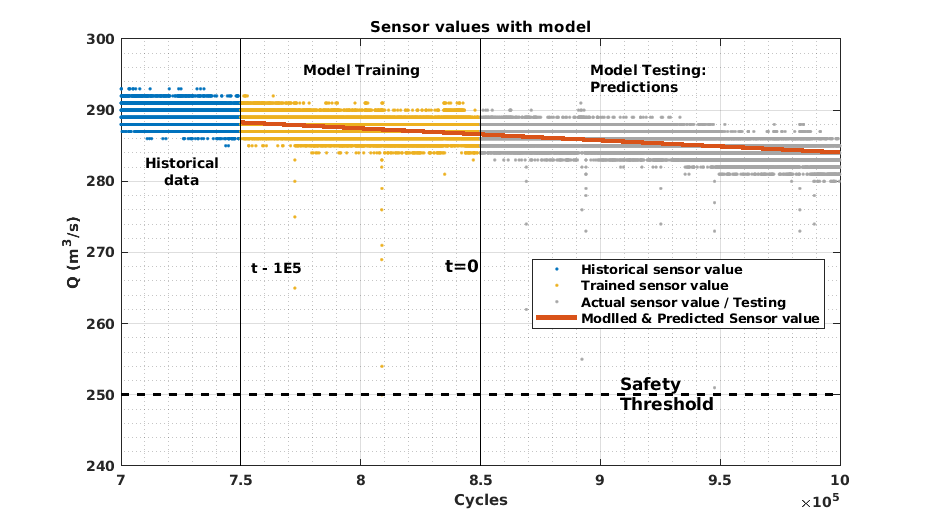
\includegraphics[width=0.7\linewidth]{Model.png}}
\caption{Sensor values of flow-rate training period of $10^5$ cycles and prediction of sensor values and RUL until the predicted values crosses the ST.}
\label{fig:Model}
\end{figure}
\section{Regressive Event-Tracker}
\label{sec:RET}
The data from the online repository is accessed via Orion context broker using FIWARE protocols. The sensor data are modelled by a linear degradation model, as described in \eqref{eq:fx}. The $f(x)$ is the model of the sensor values, $\sigma$ is the set values of any of the sensors chosen by the operator/the end-user or the manufacturer, $\phi(t)$ is the time-varying degradation model, and $\varepsilon(t)$ is the data acquisition instrumentation noise which could be a combination of Gaussian and Poissonian.
\begin{equation}
    f(x) = \sigma + \phi(t)\cdot g(t) + \varepsilon(t)
    \label{eq:fx}
\end{equation}
The noise in the model can be minimised by having a larger training period. The function $g(t)=t$, as for the case for linear models. An exponential model can also be considered; however, for fast prediction, the linear models are implementable with less computational complexity. The RUL is estimated as shown in the \eqref{eq:RUL} at every cycle and described in Fig.~\ref{fig:Model}.
\begin{equation}
    R(t) = \left(\frac{S-\sigma}{\phi(t)}\right)-t
    \label{eq:RUL}
\end{equation}
For the calculation of RUL at every cycle, $R(t)$, the ST is set at $85\%$ of the value of set value as explained in the previous section. Fig.~\ref{fig:Model} shows the implementation of regressive based predictions. The model is trained with a historical data length of $105$ cycles, and then the extrapolation of the trained model would be the prediction of the future sensor value. The time (cycles) frame between the trained cycle and the predicted sensors crossing the ST is the RUL, as shown in Fig.~\ref{fig:Model}.
\begin{figure}[t]
    \centering
  \subfloat[MTTF - Coolant flow-rate\label{1a}]{%
       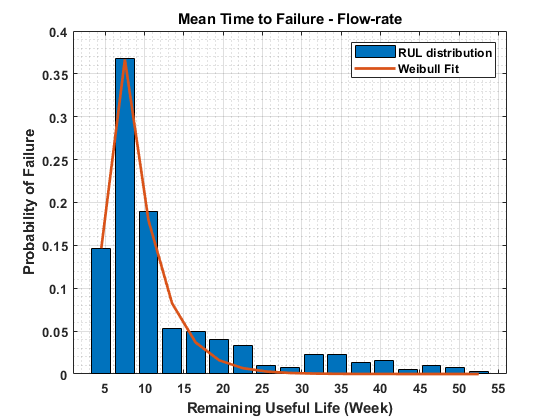
\includegraphics[width=0.45\linewidth]{MTTF_PORT_PI.png}}
    \hfill
  \subfloat[MTTF - Coolant pressure\label{1b}]{%
        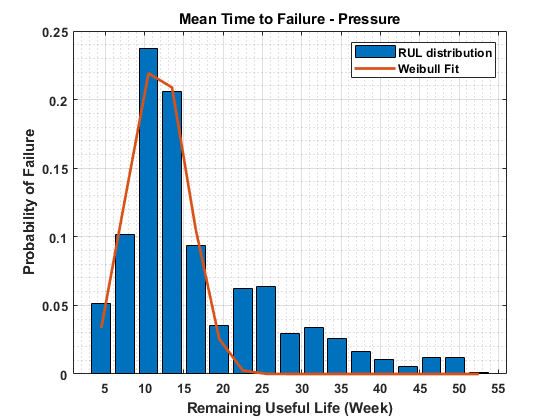
\includegraphics[width=0.45\linewidth]{MTTF_pressure1.png}}
    \\
  \subfloat[MTTF - Coolant temperature\label{1c}]{%
        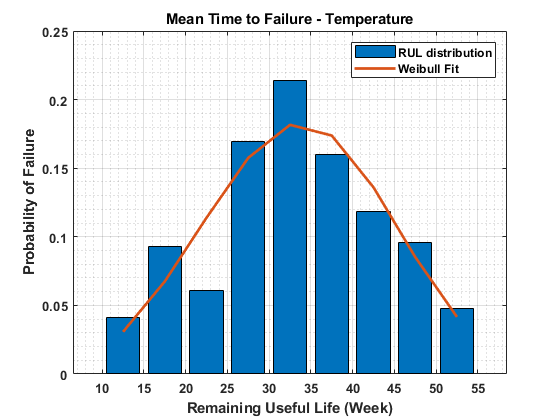
\includegraphics[width=0.45\linewidth]{MTTF_TEMP_PI.png}}
    \hfill
  \subfloat[MTTF - \% Control valve\label{1d}]{%
        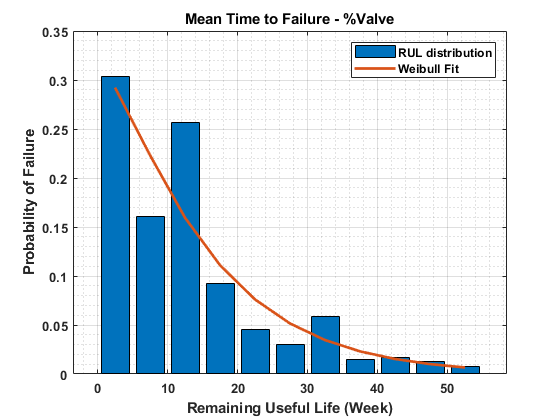
\includegraphics[width=0.45\linewidth]{MTTF_x_PI.png}}
  \caption{MTTF estimation for each sensor in the thermal regulator. The ST is $85\%$ of the set value of the sensors.}
  \label{fig:Weibull}
\end{figure}
\begin{table}[b]
    \caption{The MTTF estimation components via the associated four sensors of the thermal regulator}
    \begin{center}
        \begin{tabular}{|c|c|}
            \hline
            \textbf{Sensors}& \textbf{MTTF} \\
            \hline
            Coolant flow-rate ($R_1(t)$) & \num{9}~week  \\
            \hline
            Pressure ($R_2(t)$) & \num{10}~week \\
            \hline
            \% control valve opening ($R_4(t)$) & \num{1}~week \\
            \hline
            Temperature ($R_3(t)$) & \num{32}~week \\
            \hline
        \end{tabular}
        \label{tab:III}
    \end{center}
\end{table}
\subsection{MTTF estimation for each sensors}
\label{subsec:MTTF}
The estimation of RUL for all the sensors is carried out according to the ST prescribed by the machine manufacturer, i.e. $85\%$ of the set values. The distribution analysis of the RUL provides the insight of mean time for the machine to be in optimum regime conditions. The Weibull distribution which, as shown in Fig.~\ref{fig:Weibull} of all the sensors in the thermal regulator. If the ST can be considered as the definite filter clog failure threshold, then the mean time of the operations becomes an MTTF, and the RUL becomes time to failure. The estimated MTTF for sensors is shown in Table~\ref{tab:III}.

\subsection{Estimation of lifetime of the thermal regulator}
\label{subsec:Lifetime}
The life-time, $R_{eff} (t)$, of the thermal regulator with respect to the filter clog failure mode is estimated by the combination of MTTF of all the sensors and the weightage ($w$) of the sensors related to the filter clog as estimated in Table~\ref{tab:I}. The life time of the thermal regulator is estimated as shown in \eqref{eq:R_eff}.
\begin{equation}
    R_{eff}(t) = \frac{\sum\limits_{i=1}^N w_i R_i(t)}{\sum\limits_{i=1}^N w_i}
    \label{eq:R_eff}
\end{equation}
Where $R_N (t)$ and $N$ are the MTTF and number of sensors in the thermal regulator, the estimated life-time of the thermal regulator with respect to filter clog is $12$~week \SI{3}{\day} \SI{16}{\hour} \SI{25}{\minute} \SI{15}{\second}. The life-time of the thermal regulator estimation clearly dependent on the safety (failure) threshold.

\section{Conclusion}
\label{sec:conclusion}
This paper proposed a new framework for real-time sequencing strategy predicts of machine breakdown and combining it with more traditional ML techniques such as regressive methodology along with Weibull failure-rate analysis. The Theory of GMB’s term was instigated from genetic science and DNA forms to label and establish sequential event differentiation. These labelled genomes of the machine states are being used to predict the events according to their occurrence sequence, which leads to predict machine breakdown. An industrial case study of continuous compression moulding machine manufactures the plastic bottle closure (caps) in beverage industry has been considered as an experiment to predict the machine breakdown. This case study also has been applied in the proposed Regression Event-Tracker method to estimates the condition monitoring of the components and provide real-time RUL estimation. The methodology also provides the life-time of the thermal regulator based on the sensors' weighting obtained from event-clustering and MTTF estimation of each sensor. A schematic of the applied research work process on the case study, including the data acquisition system, two raw sensor signals, breakdown prediction and RUL estimation and ultimately, decision making is illustrated in Fig.~\ref{fig:Schematic_applied_work}.  The more details of the proposed method as well as validation and verification through comparison of its accuracy with other ML and DL techniques still have the potential for further research.
\begin{figure}[htbp]
\centerline{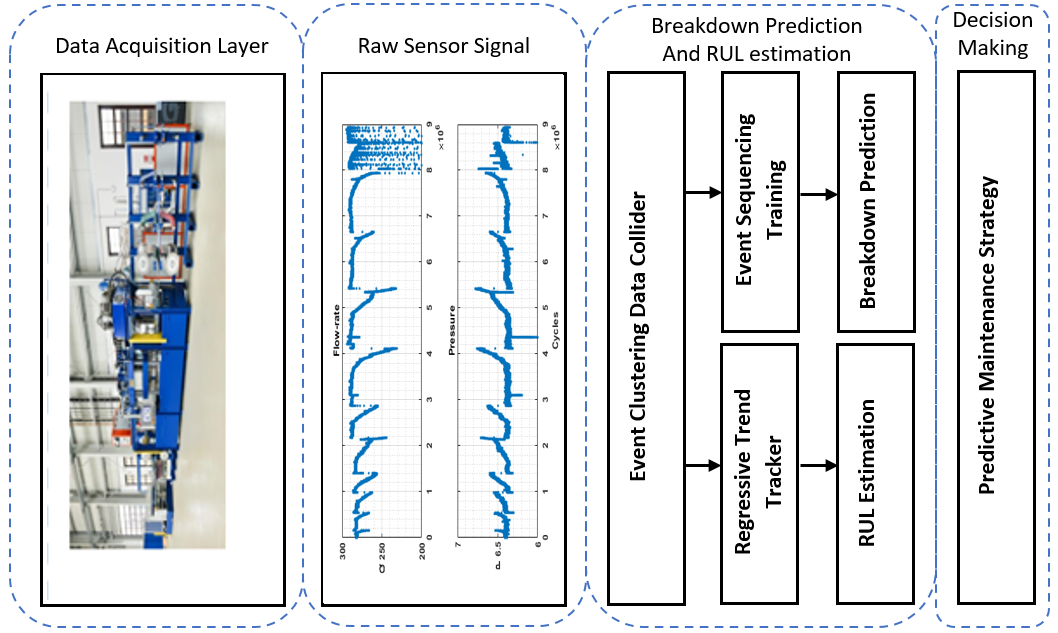
\includegraphics[width=\linewidth]{Overall.png}}
\caption{A schematic of the applied research work process on the case study.}
\label{fig:Schematic_applied_work}
\end{figure}

\bibliographystyle{IEEEtran}
\bibliography{IEEEbib}

\end{document}
